\documentclass[conference]{IEEEtran}

\usepackage{amsmath}
\usepackage{booktabs}
\usepackage{graphicx}
\usepackage{hyperref}
\usepackage{xcolor}
\usepackage{array}
\usepackage{tabularx}
\usepackage{placeins}

\graphicspath{{../plots/}}
\IfFileExists{generated_results.tex}{% This file is generated by scripts/generate_report_assets.py.
\newcommand{\TaskOneMacro}{0.2863}
\newcommand{\TaskOneMicro}{0.4000}
\newcommand{\TaskOneAUC}{0.2979}
  \newcommand{\TaskTwoGNNFone}{0.3364}
  \newcommand{\TaskTwoCNNFone}{0.7859}
  \newcommand{\TaskTwoGNNAccuracy}{0.3495}
  \newcommand{\TaskTwoCNNAccuracy}{0.7864}
\newcommand{\TaskThreeCrossFone}{0.3786}
\newcommand{\TaskThreeCrossAUC}{0.3545}
\newcommand{\TaskThreeConcatFone}{0.3708}
\newcommand{\TaskThreeConcatAUC}{0.3541}
\newcommand{\MusicCapsTrain}{2396}
\newcommand{\MusicCapsValidation}{267}
\newcommand{\MusicCapsTest}{2858}
\newcommand{\MTATTrain}{18706}
\newcommand{\MTATValidation}{1825}
\newcommand{\MTATTest}{5329}
\newcommand{\TaskFourTrain}{364}
\newcommand{\TaskFourValidation}{89}
\newcommand{\TaskFourTest}{93}
\newcommand{\TaskFourCtoAOne}{0.0215}
\newcommand{\TaskFourCtoAFive}{0.0968}
\newcommand{\TaskFourCtoATen}{0.1720}
\newcommand{\TaskFourAtoCOne}{0.0430}
\newcommand{\TaskFourAtoCFive}{0.1398}
\newcommand{\TaskFourAtoCTen}{0.2151}
\newcommand{\TaskFourRandomFive}{0.0538}
\newcommand{\TaskFourBestEpoch}{22}
\newcommand{\TaskFourZeroShotMacro}{0.0111}
\newcommand{\TaskFourTaskThreeMacro}{0.0500}
  \newcommand{\EvaluationTableRows}{%
Random tags (MTAT) & -- & 0.1107 & 0.0662 & -- \\
Task 1: DistilBERT & -- & 0.2863 & 0.2979 & -- \\
Task 2: GraphSAGE & 0.3495 & 0.3364 & -- & -- \\
Task 2: CNN & 0.7864 & 0.7859 & -- & -- \\
Task 3: BERT only & -- & 0.2812 & 0.2525 & -- \\
Task 3: GNN only & -- & 0.2967 & 0.2442 & -- \\
Task 3: Concatenation & -- & 0.3708 & 0.3541 & -- \\
Task 3: Cross-attention & -- & 0.3786 & 0.3545 & -- \\
Task 4: Contrastive & -- & -- & -- & 0.0968 \\
  }
  \newcommand{\TaskOneExampleRows}{%
The low quality recording features a ballad song that contains sustained strings, mellow piano melody and soft f... & low quality, soulful, sustained strings melody, sad & emotional, passionate, low quality, mellow \\
a male voice is singing a melody with changing tempos while snipping his fingers rhythmically. The recording sou... & amateur recording, reverb & uptempo, medium tempo, amateur recording, medium to uptempo \\
This song contains digital drums playing a simple groove along with two guitars. One strumming chords along with... & medium tempo, piano, acoustic guitar, e-bass & acoustic drums, e-bass, piano, medium to uptempo \\
  }
}{
  \newcommand{\TaskOneMacro}{--}
  \newcommand{\TaskOneMicro}{--}
  \newcommand{\TaskOneAUC}{--}
  \newcommand{\TaskTwoGNNFone}{--}
  \newcommand{\TaskTwoCNNFone}{--}
  \newcommand{\TaskTwoGNNAccuracy}{--}
  \newcommand{\TaskTwoCNNAccuracy}{--}
  \newcommand{\TaskThreeCrossFone}{--}
  \newcommand{\TaskThreeCrossAUC}{--}
  \newcommand{\TaskThreeConcatFone}{--}
  \newcommand{\TaskThreeConcatAUC}{--}
  \newcommand{\MusicCapsTrain}{--}
  \newcommand{\MusicCapsValidation}{--}
  \newcommand{\MusicCapsTest}{--}
  \newcommand{\MTATTrain}{--}
  \newcommand{\MTATValidation}{--}
  \newcommand{\MTATTest}{--}
  \newcommand{\TaskFourTrain}{--}
  \newcommand{\TaskFourValidation}{--}
  \newcommand{\TaskFourTest}{--}
  \newcommand{\TaskFourCtoAOne}{--}
  \newcommand{\TaskFourCtoAFive}{--}
  \newcommand{\TaskFourCtoATen}{--}
  \newcommand{\TaskFourAtoCOne}{--}
  \newcommand{\TaskFourAtoCFive}{--}
  \newcommand{\TaskFourAtoCTen}{--}
  \newcommand{\TaskFourRandomFive}{--}
  \newcommand{\TaskFourBestEpoch}{--}
  \newcommand{\TaskFourZeroShotMacro}{--}
  \newcommand{\TaskFourTaskThreeMacro}{--}
  \newcommand{\EvaluationTableRows}{Results not generated & -- & -- & -- & -- \\
  }
  \newcommand{\TaskOneExampleRows}{Results not generated & -- & -- \\
  }
}

\title{GNN-Based BERT for Understanding Context from Music}
\author{
\IEEEauthorblockN{
\begin{tabular}{cc}
Kazi Salman Salim & Miskatul Afrin Anika
\end{tabular}}
\IEEEauthorblockA{
\begin{tabular}{cc}
Student ID: 23101209 & Student ID: 23101409 \\
Section: 3 & Section: 3
\end{tabular}\\
Course: CSE425 --- Neural Networks\\
Course Instructor: Moin Mostakim}}

\begin{document}
\maketitle

\begin{abstract}
This project studies music-context prediction using text and audio structure. DistilBERT is
used to encode captions or tag-based context, while GraphSAGE encodes graphs whose nodes are
short audio segments. Three required experiments are evaluated: a text-only MusicCaps tag
classifier, an audio-only GraphSAGE model compared with a spectrogram CNN on GTZAN, and a
  four-way GNN--BERT ablation on MagnaTagATune. A fourth experiment trains a contrastive
  audio--caption model on recovered real MusicCaps intervals and evaluates bidirectional retrieval.
  The implementation uses frozen data splits, validation-only model selection, and saved evaluation
  artifacts. The main goal is not to claim
state-of-the-art performance, but to test whether graph and text representations provide
complementary information under a reproducible experimental setup.
\end{abstract}

\section{Introduction}
Music context includes genre, mood, instrumentation, rhythm, and the words people use to
describe a recording. A spectrogram CNN can learn local time--frequency patterns, but it does
not directly model relationships between distant parts of a track. A graph provides a simple
way to represent those relationships: each node is an audio segment and edges represent either
temporal adjacency or acoustic similarity. Text encoders provide a second view of the same
recording through captions or tags.

The project follows the supplied CSE425 assignment. Task 1 tests a BERT baseline, Task 2 tests
an audio graph, and Task 3 combines both modalities. The main research question is whether the
fusion models improve over their single-modality ablations. Task 4 is treated as an advanced
extension because MusicCaps audio must be recovered from external YouTube links and some clips
may no longer be available.
\subsection{Relation to the CSE425 Course Outline}
The work also follows the supplied CSE425 Neural Networks course outline. It applies CNNs to
log-mel spectrograms, transformer attention through DistilBERT, transfer learning through
pretrained text weights, and AdamW optimization with gradient clipping, dropout, learning-rate
scheduling, and early stopping. Ablations, confusion matrices, per-tag scores, and attention
visualizations support model interpretation and transparent comparison. The GNN is a
project-specific architecture required by the separate project brief. Together, the stages form
an end-to-end workflow covering data preparation, training, validation, evaluation, and
explainability.


\section{Datasets and Splits}
\subsection{MusicCaps}
MusicCaps contains 5,521 expert-written music captions. Rows marked as AudioSet evaluation
examples are held out as the test set. The remaining rows are split deterministically into
90\% training and 10\% validation data. This gives \MusicCapsTrain{} training,
\MusicCapsValidation{} validation, and \MusicCapsTest{} test examples. The Task 1 label
vocabulary is built from the training split only, with a minimum frequency of 20.

\subsection{GTZAN}
GTZAN contains ten genres with approximately 100 tracks per genre. One unreadable track is
excluded during preprocessing and recorded in the preprocessing report. Because GTZAN contains
repeated files, SHA-256 hashes are used as group identifiers during a seeded, per-genre split.
All copies of identical audio remain in one partition. The split audit found 14 duplicate groups
and zero groups crossing train, validation, and test. Both Task 2 models use exactly the same IDs.

\subsection{MagnaTagATune}
MagnaTagATune contains 29-second audio clips with binary tags. The official archive-shard
protocol is used: shards 0--b are training, shard c is validation, and shards d--f are test.
After checking usable graph files, Task 3 contains \MTATTrain{} training,
\MTATValidation{} validation, and \MTATTest{} test clips. Exact clip overlap and exact
$(\text{artist},\text{title},\text{album})$ overlap are zero. Some artist overlap remains and
is reported in the split audit rather than being hidden.

\section{Preprocessing}
All audio is loaded as mono and resampled to 22,050 Hz. For the CNN, a 128-bin log-mel
spectrogram is computed and normalized per track. Graph nodes use non-overlapping five-second
segments. Each node has 77 summary features: MFCC means and standard deviations, chroma means
and standard deviations, spectral contrast, spectral centroid, zero-crossing rate, and RMS
energy. Features are standardized within each track.

For node features $x_i$ and $x_j$, an acoustic edge is added when
\begin{equation}
  \frac{x_i^\top x_j}{\lVert x_i\rVert\lVert x_j\rVert} > \tau,
\end{equation}
where $\tau=0.5$. Consecutive segments are always connected in both directions, and self-loops
are added. Every saved graph is checked for non-finite features, empty node sets, and invalid
edge indices. A graph coherence score $S=\frac{1}{|E'|}\sum_{(i,j)\in E'}\mathbf{1}[\cos(x_i,x_j)>\tau]$
is also computed over non-self-loop edges. Across GTZAN and MTAT, coherence averages 0.012 and
0.030 respectively, confirming that most edges are temporal-adjacency links between acoustically
distinct segments rather than similarity-based shortcuts.

Text is tokenized with the uncased DistilBERT tokenizer. Task 1 uses the expert caption. Task 3
constructs a short sentence from 31 instrument/vocal context tags. The 19 prediction targets
contain 12 genre and 7 mood tags. The two tag sets are lexically disjoint. They still come from
the same annotation process, so indirect statistical relationships are possible.

\section{Models}
\subsection{Task 1: BERT Baseline}
The DistilBERT representation of the first token is passed through a two-layer classifier. For
target vector $y$ and logits $s$, training uses binary cross-entropy with logits. Class weights
are calculated from training labels only. The classifier head is trained first with the BERT
backbone frozen, followed by full-backbone fine-tuning.

\subsection{Task 2: GraphSAGE and CNN}
The GNN uses three GraphSAGE layers with 256 hidden units, followed by global mean pooling and a classification head.
For graph $G$ with final node states $h_i$, the graph representation is
\begin{equation}
  g=\frac{1}{|V|}\sum_{i\in V}h_i.
\end{equation}
The comparison model is a three-block convolutional network over the normalized log-mel
spectrogram. Both models use cross-entropy loss and validation Macro-F1 for checkpoint selection.

\subsection{Task 3: GNN--BERT Fusion}
Four conditions are trained: BERT only, GNN only, early concatenation, and cross-attention.
For cross-attention, the graph embedding is the query and DistilBERT token embeddings are keys
and values:
\begin{align}
  Q &= gW_Q, & K &= H_{text}W_K, & V &= H_{text}W_V,\\
  A &= \operatorname{softmax}\left(\frac{QK^\top}{\sqrt{d}}\right),\\
  z &= [g;AV].
\end{align}
The fused vector $z$ is passed to a multi-label classifier. Padding positions are masked before
the softmax. BERT is first frozen and then its last transformer layer is fine-tuned.

\IfFileExists{../plots/task3_architecture.png}{
\begin{figure*}[t]
  \centering
  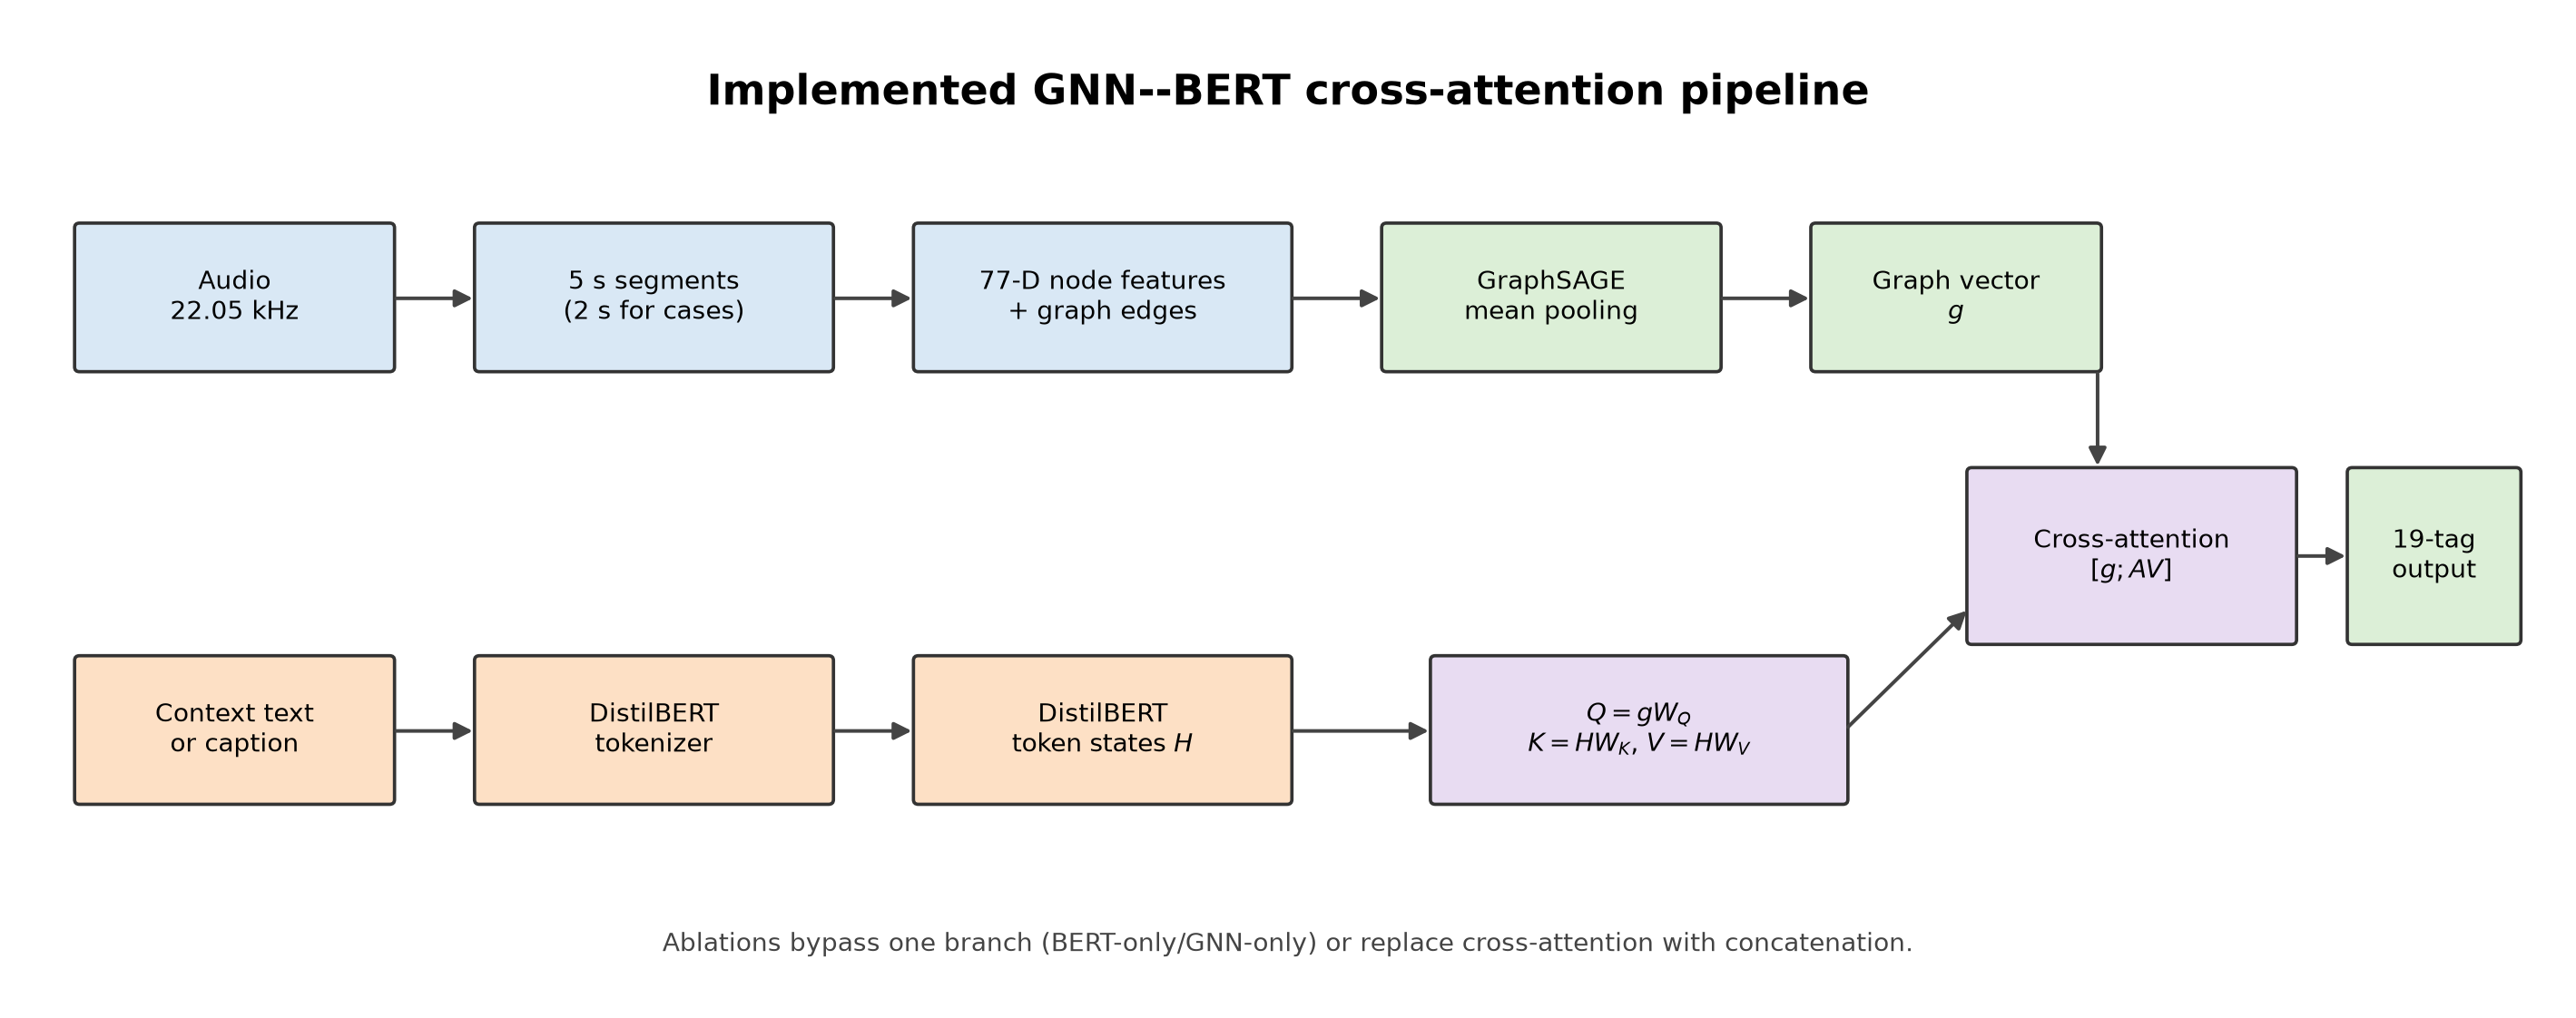
\includegraphics[width=.96\textwidth]{task3_architecture.png}
  \caption{Implemented audio-graph and text cross-attention pipeline.}
\end{figure*}}{}

\subsection{Task 4: Contrastive Extension}
The extension projects GraphSAGE and caption encodings into a shared 128-dimensional normalized
space and uses a symmetric InfoNCE loss. DistilBERT is frozen, while GraphSAGE is initialized
from the Task 3 audio encoder. It is evaluated with caption-to-audio and audio-to-caption
Recall@1, Recall@5, and Recall@10.

\section{Experimental Setup}
Experiments use seed 42. AdamW, gradient clipping, and early stopping are used for all neural
models. Classification checkpoints are selected with validation Macro-F1. Task 4 instead uses
mean bidirectional validation Recall@5. A global multi-label threshold
is then selected on validation predictions and applied once to test predictions. The report
uses Macro-F1, Micro-F1, and mean per-tag AUC-PR. GTZAN additionally reports accuracy and a
confusion matrix.

\subsection{Training and Fine-Tuning Procedure}
The same validation-first procedure is used for each model. First, the fixed split is loaded and
class weights are calculated from training labels only. For every epoch, the model is updated on
training batches, then evaluated on the validation partition. The checkpoint is replaced only
when validation Macro-F1 improves, and early stopping ends a run after the stated patience. For a
multi-label task, the best checkpoint produces validation probabilities used to choose one global
decision threshold. Finally, that frozen checkpoint and threshold are evaluated once on the test
partition. This order prevents test labels from influencing training, checkpoint selection, or
threshold selection.

For Task 4, the requested MusicCaps ranges are frozen before the final run: records 0--399 of
the training split, 0--99 of validation, and 200--299 of the official test split. Clips whose
source video cannot be recovered are omitted without replacement. This leaves
\TaskFourTrain{}/\TaskFourValidation{}/\TaskFourTest{} usable real graph--caption pairs. The
final test block was not used by the earlier feasibility run and is evaluated only after
validation selects the checkpoint.

For DistilBERT fine-tuning, the transformer is initially frozen while the new prediction head and,
for Task 3, the graph/fusion modules learn. The best frozen-stage checkpoint is reloaded before
fine-tuning. Task 1 then updates the full backbone at learning rate $2\times10^{-5}$; Task 3 updates
only the final transformer layer at the same learning rate. Gradients are clipped to norm 1.0.
This two-stage schedule was used because full transformer training from the first epoch was less
stable on the available GPU.

\section{Results}
\begin{table}[t]
\centering
\caption{Main evaluation table. Dashes indicate metrics that do not apply.}
\begin{tabular}{lcccc}
\toprule
Model & Accuracy & Macro-F1 & AUC-PR & R@5\\
\midrule
\EvaluationTableRows
\bottomrule
\end{tabular}
\label{tab:main-results}
\end{table}

\subsection{Task 1}
The Task 1 test scores are Macro-F1 \TaskOneMacro{}, Micro-F1 \TaskOneMicro{}, and mean
AUC-PR \TaskOneAUC{}. The difference between Macro-F1 and Micro-F1 is expected because the
MusicCaps proxy vocabulary remains imbalanced even after the frequency filter.

\IfFileExists{../plots/task1_f1_curves.png}{
\begin{figure}[t]
  \centering
  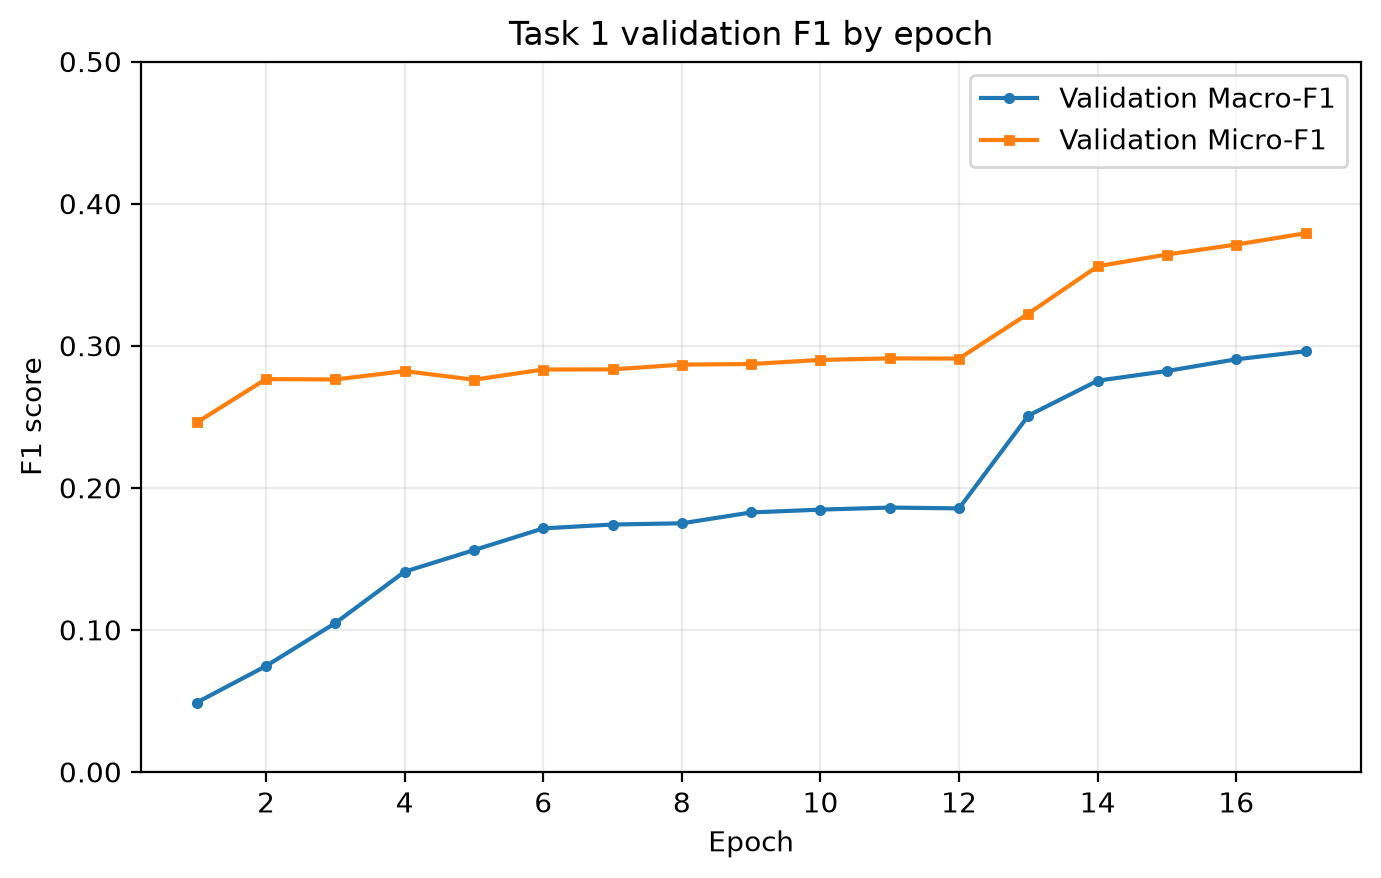
\includegraphics[width=\columnwidth]{task1_f1_curves.png}
  \caption{Task 1 validation Macro-F1 and Micro-F1 across epochs.}
\end{figure}}{}

\begin{table*}[t]
\centering
\caption{First three held-out Task 1 predictions in frozen test order. Predicted tags are the four
highest-probability outputs; true tags are limited to the training-derived vocabulary.}
\begin{tabularx}{\textwidth}{>{\raggedright\arraybackslash}X p{.22\textwidth} p{.22\textwidth}}
\toprule
Caption excerpt & True tags & Top predicted tags\\
\midrule
\TaskOneExampleRows
\bottomrule
\end{tabularx}
\end{table*}

\IfFileExists{../plots/task1_attention_example_1.png}{
\begin{figure*}[t]
  \centering
  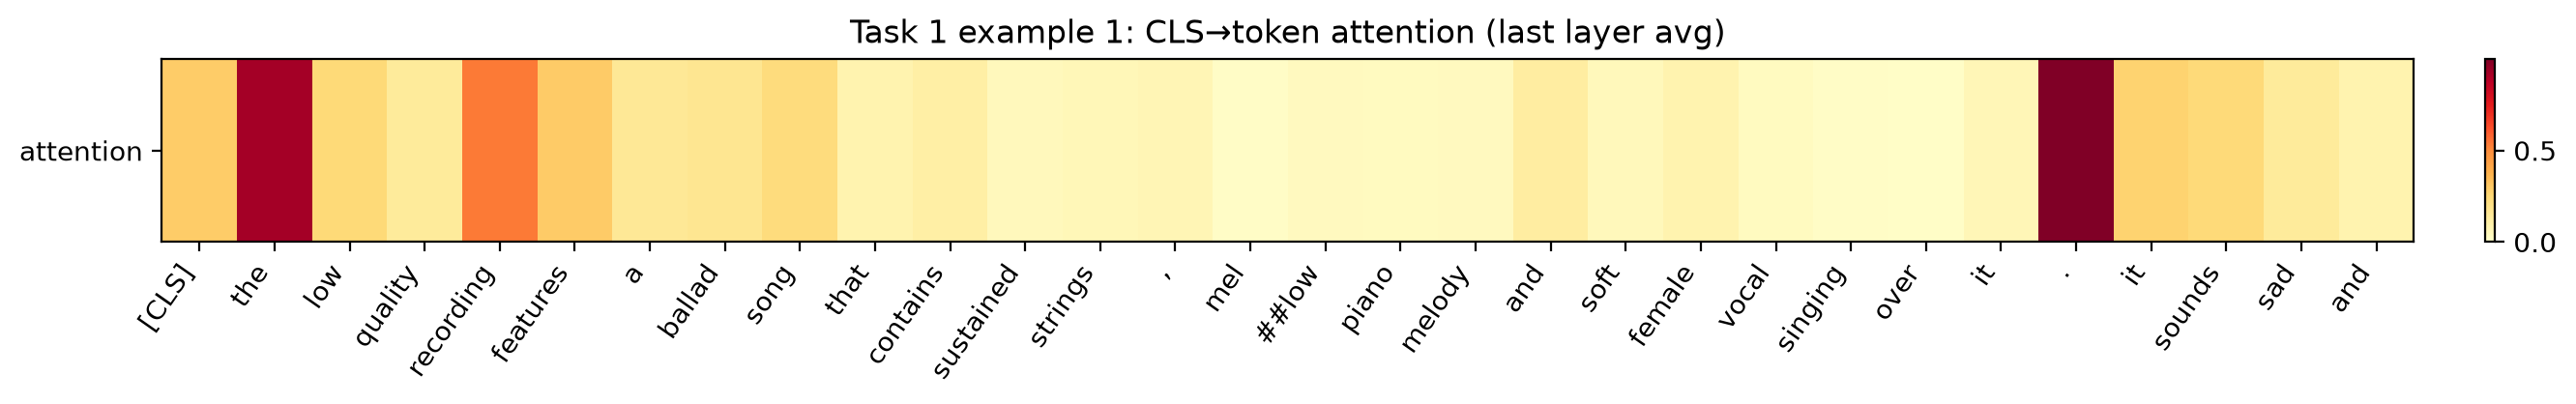
\includegraphics[width=.48\textwidth]{task1_attention_example_1.png}\hfill
  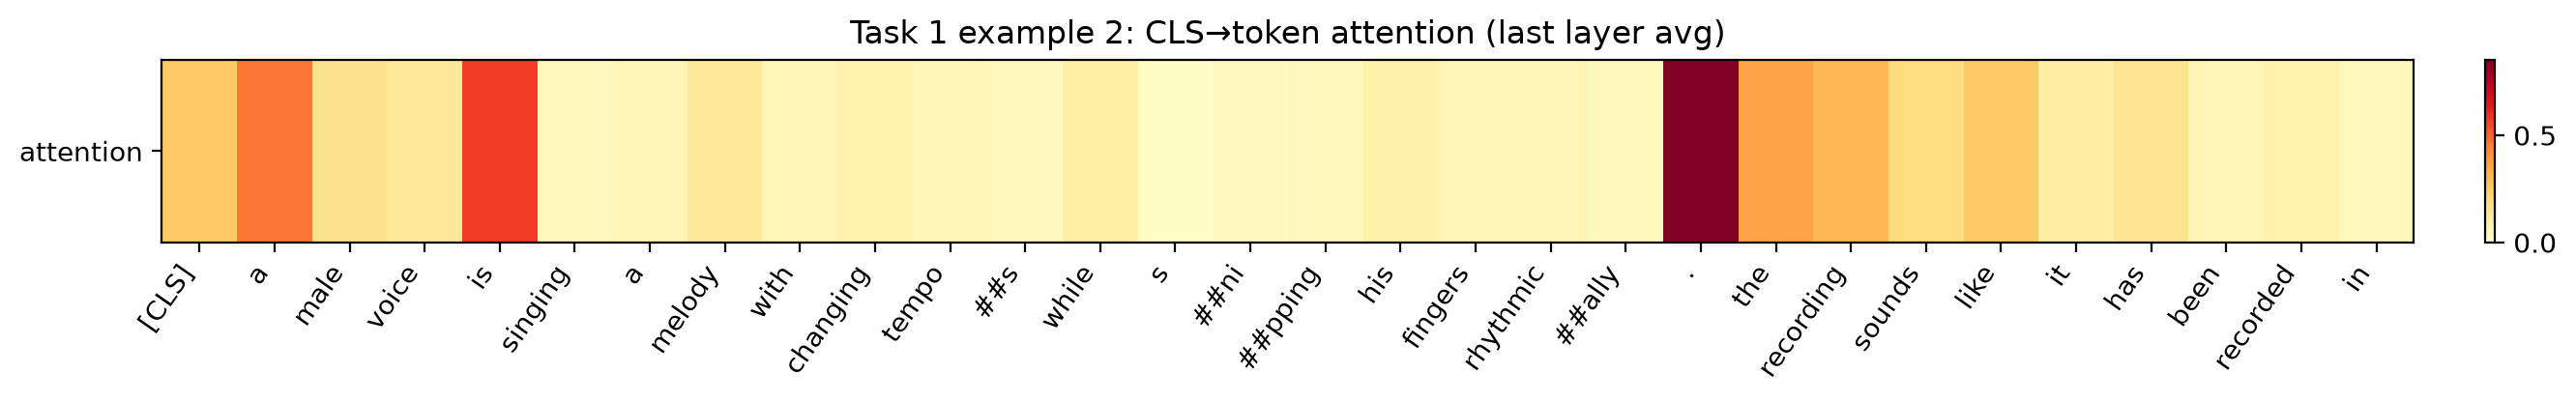
\includegraphics[width=.48\textwidth]{task1_attention_example_2.png}
  \caption{CLS-to-token attention (last-layer head average) for two held-out Task 1 captions.
  Higher intensity indicates tokens receiving more attention from the classification token.
  The model attends most to genre and mood descriptors.}
\end{figure*}}{}

\subsection{Task 2}
GraphSAGE obtains accuracy \TaskTwoGNNAccuracy{} and Macro-F1 \TaskTwoGNNFone{}, while the CNN
obtains accuracy \TaskTwoCNNAccuracy{} and Macro-F1 \TaskTwoCNNFone{}.
As an additional baseline, a PCA+MLP model is trained on aggregated hand-crafted node features
(mean, standard deviation, min, max of the 77-D segment vectors). It achieves only 11.7\%
accuracy and 0.12 Macro-F1, confirming that both the GNN and CNN architectures learn
meaningful representations beyond what a shallow classifier can extract from the same features.
The confusion matrices show which genres account for the model difference. This comparison also
tests a limitation of the graph representation: reducing a five-second segment to summary
statistics discards more local detail than the full spectrogram.

\IfFileExists{../plots/task2_model_comparison.png}{
\begin{figure}[t]
  \centering
  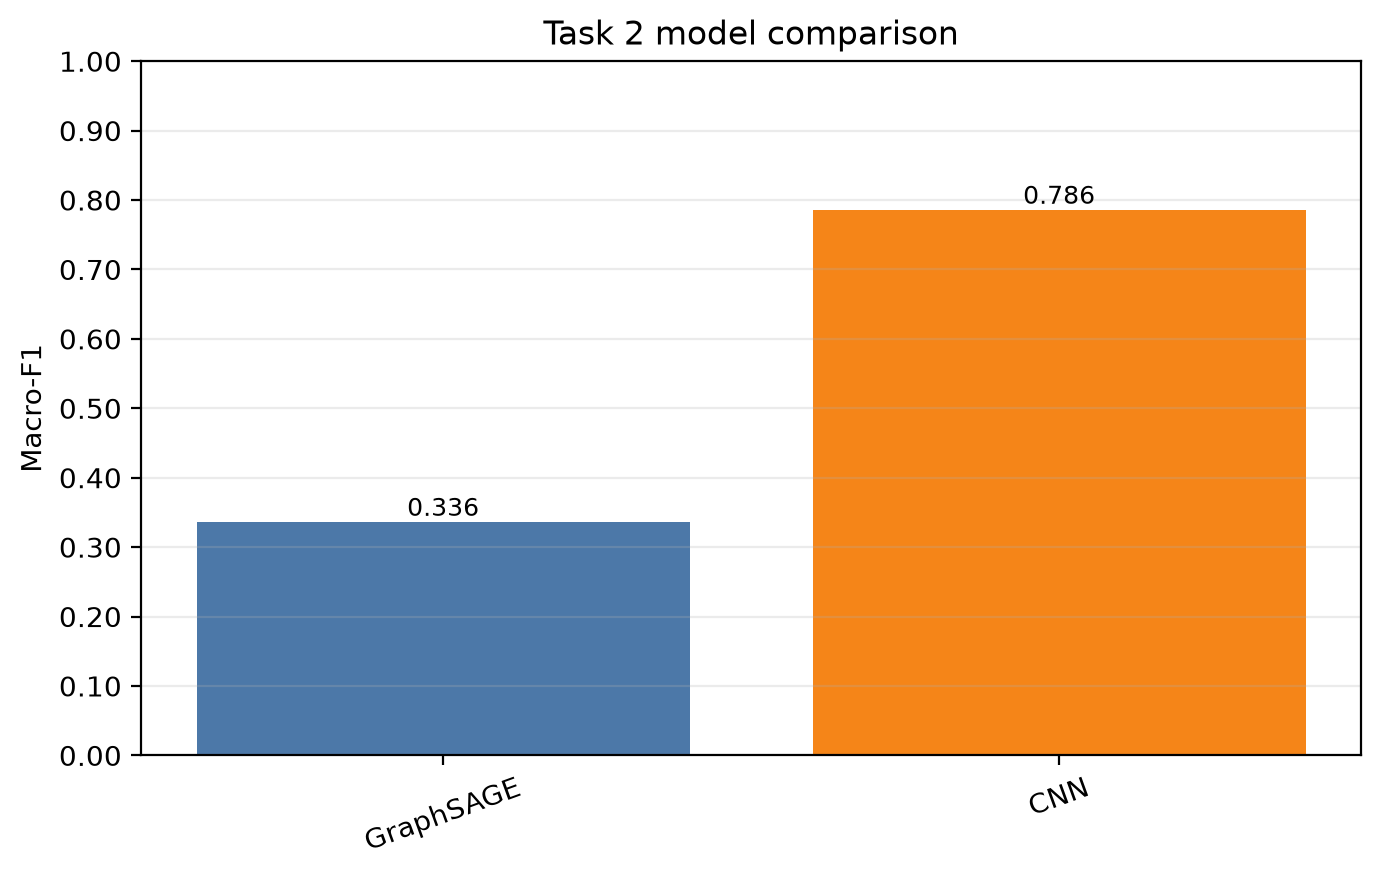
\includegraphics[width=\columnwidth]{task2_model_comparison.png}
  \caption{Task 2 Macro-F1 comparison using the same GTZAN split.}
\end{figure}}{}

\IfFileExists{../plots/task2_cnn_confusion_matrix.png}{
\begin{figure*}[t]
  \centering
  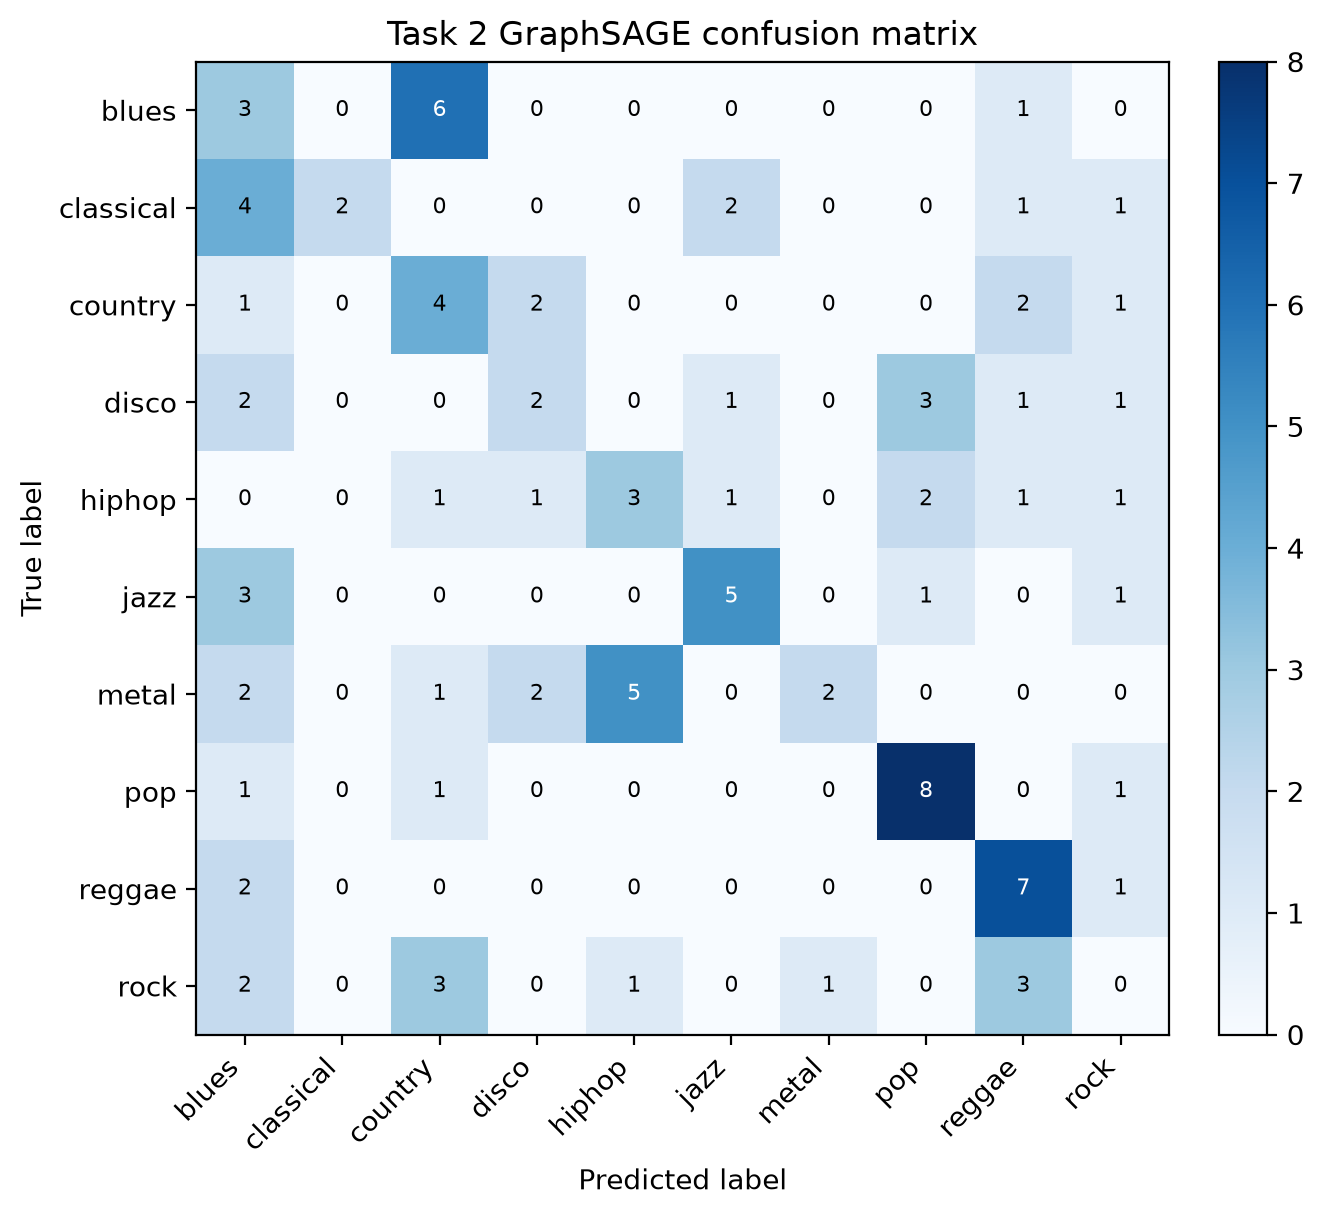
\includegraphics[width=.45\textwidth]{task2_gnn_confusion_matrix.png}\hfill
  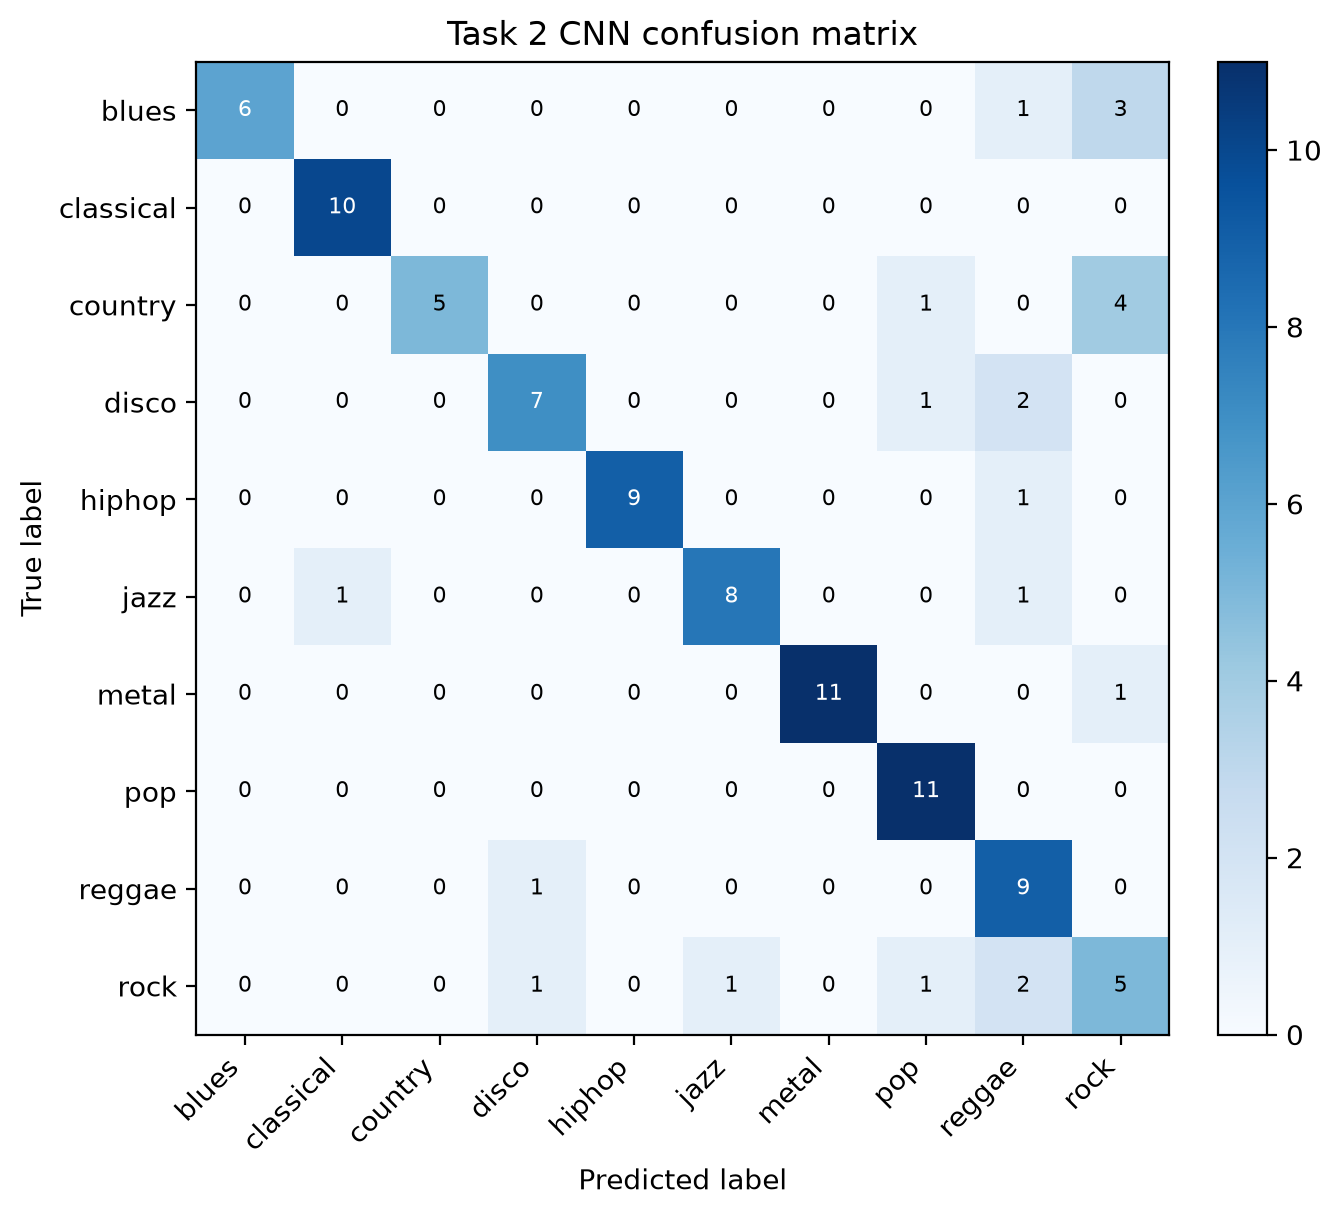
\includegraphics[width=.45\textwidth]{task2_cnn_confusion_matrix.png}
  \caption{Task 2 test confusion matrices for GraphSAGE (left) and CNN (right).}
\end{figure*}}{}

\subsection{Task 3}
Early concatenation gives the highest held-out result, with Macro-F1 \TaskThreeConcatFone{} and
mean AUC-PR \TaskThreeConcatAUC{}. Cross-attention is second with Macro-F1
\TaskThreeCrossFone{} and mean AUC-PR \TaskThreeCrossAUC{}. Both fusion models improve over
the BERT-only and GNN-only conditions, which supports the claim that their information is
complementary. However, cross-attention does not improve over simple concatenation. A likely
reason is that the context sentences are short, templated lists of tags, so pooled features are
already informative and the additional attention parameters do not provide a consistent benefit.
Per-tag results are retained because an average score can hide weak performance on rare labels.

\IfFileExists{../plots/task3_ablation_macro_f1.png}{
\begin{figure*}[t]
  \centering
  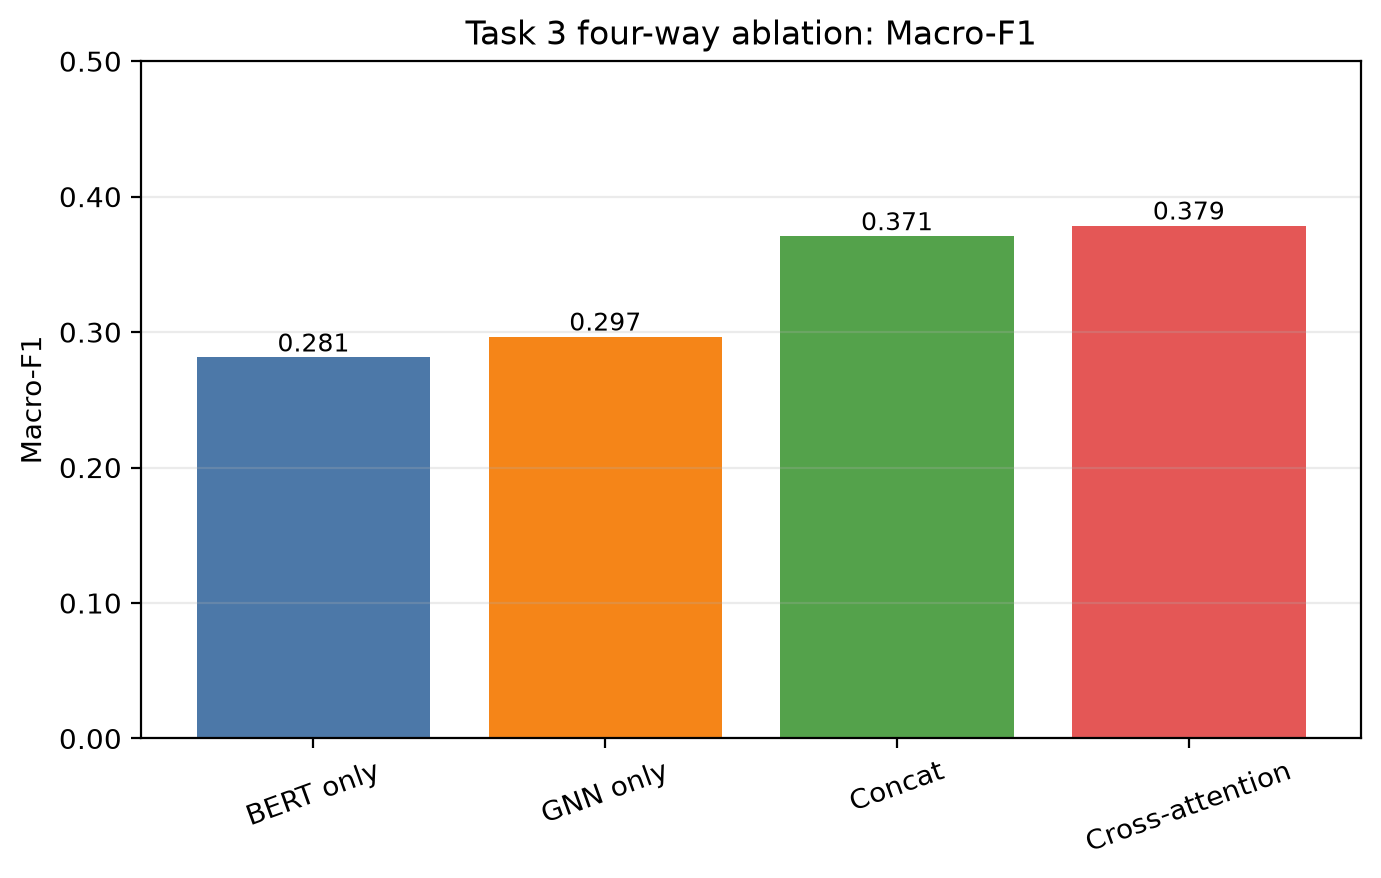
\includegraphics[width=.47\textwidth]{task3_ablation_macro_f1.png}\hfill
  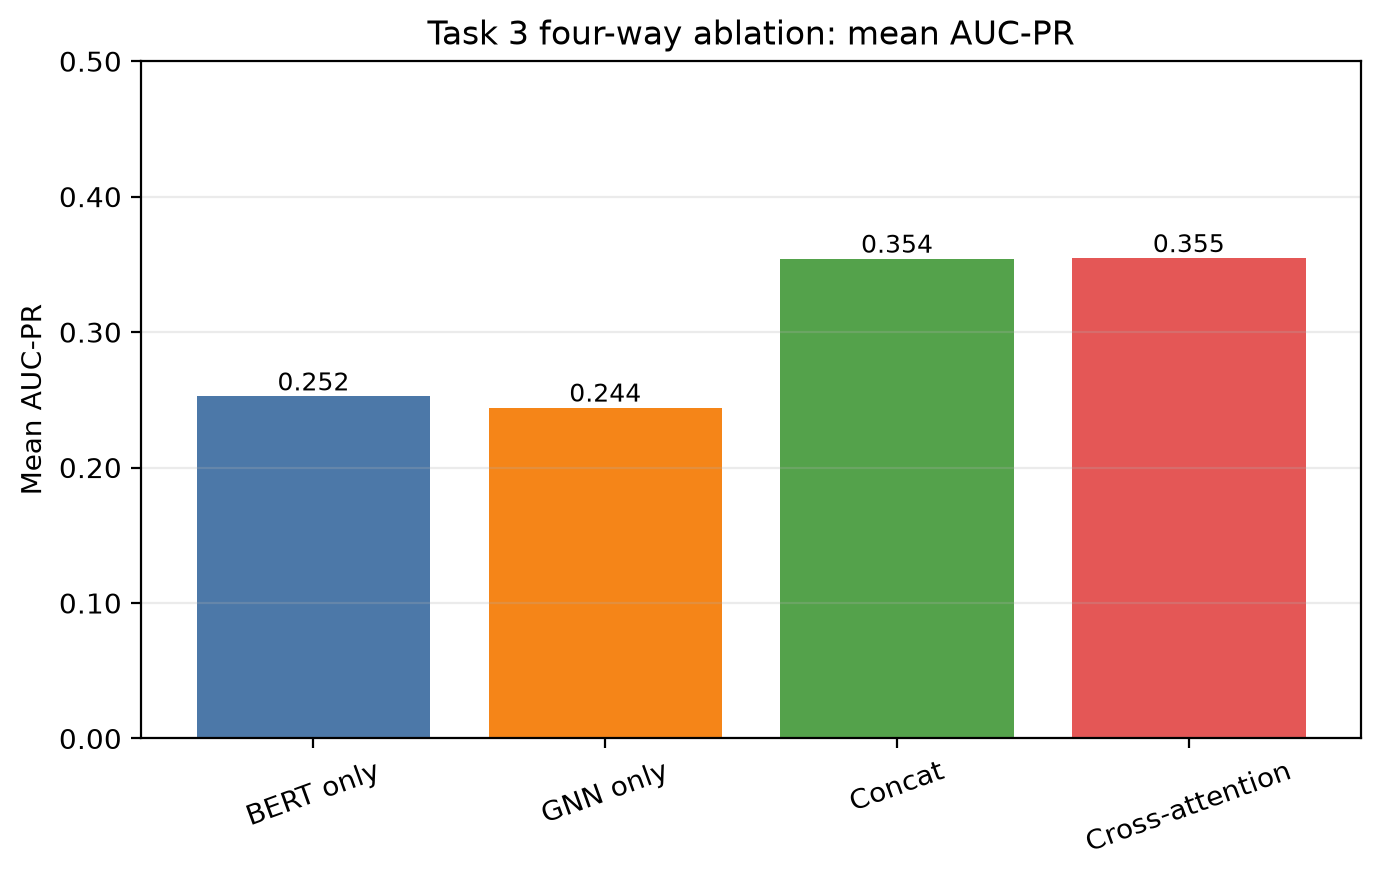
\includegraphics[width=.47\textwidth]{task3_ablation_auc_pr.png}
  \caption{Task 3 four-way ablation measured by Macro-F1 and mean AUC-PR.}
\end{figure*}}{}

\IfFileExists{../plots/task3_per_tag_metrics.png}{
\begin{figure*}[t]
  \centering
  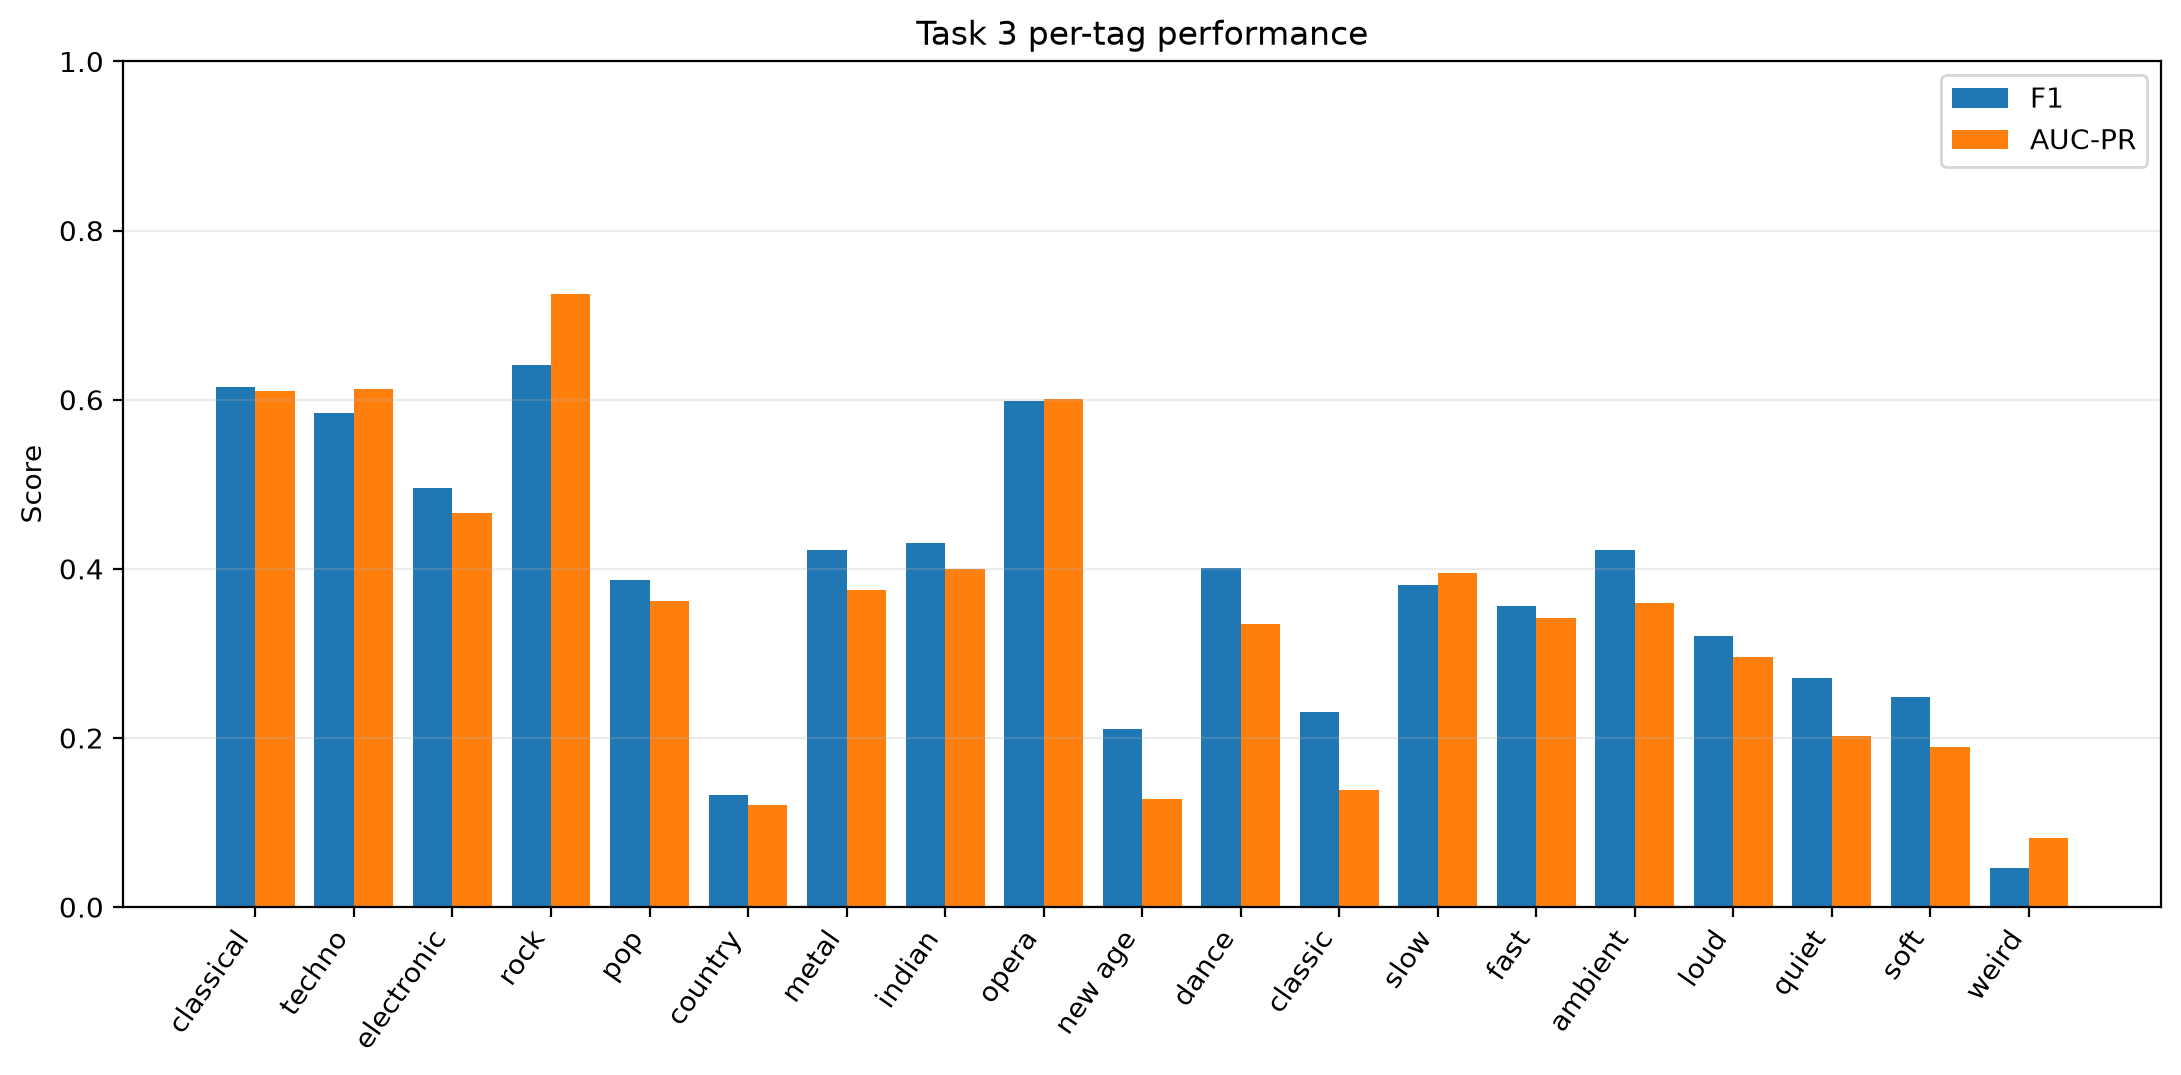
\includegraphics[width=.48\textwidth]{task3_per_tag_metrics.png}\hfill
  \begin{minipage}[c]{.48\textwidth}
    \centering
    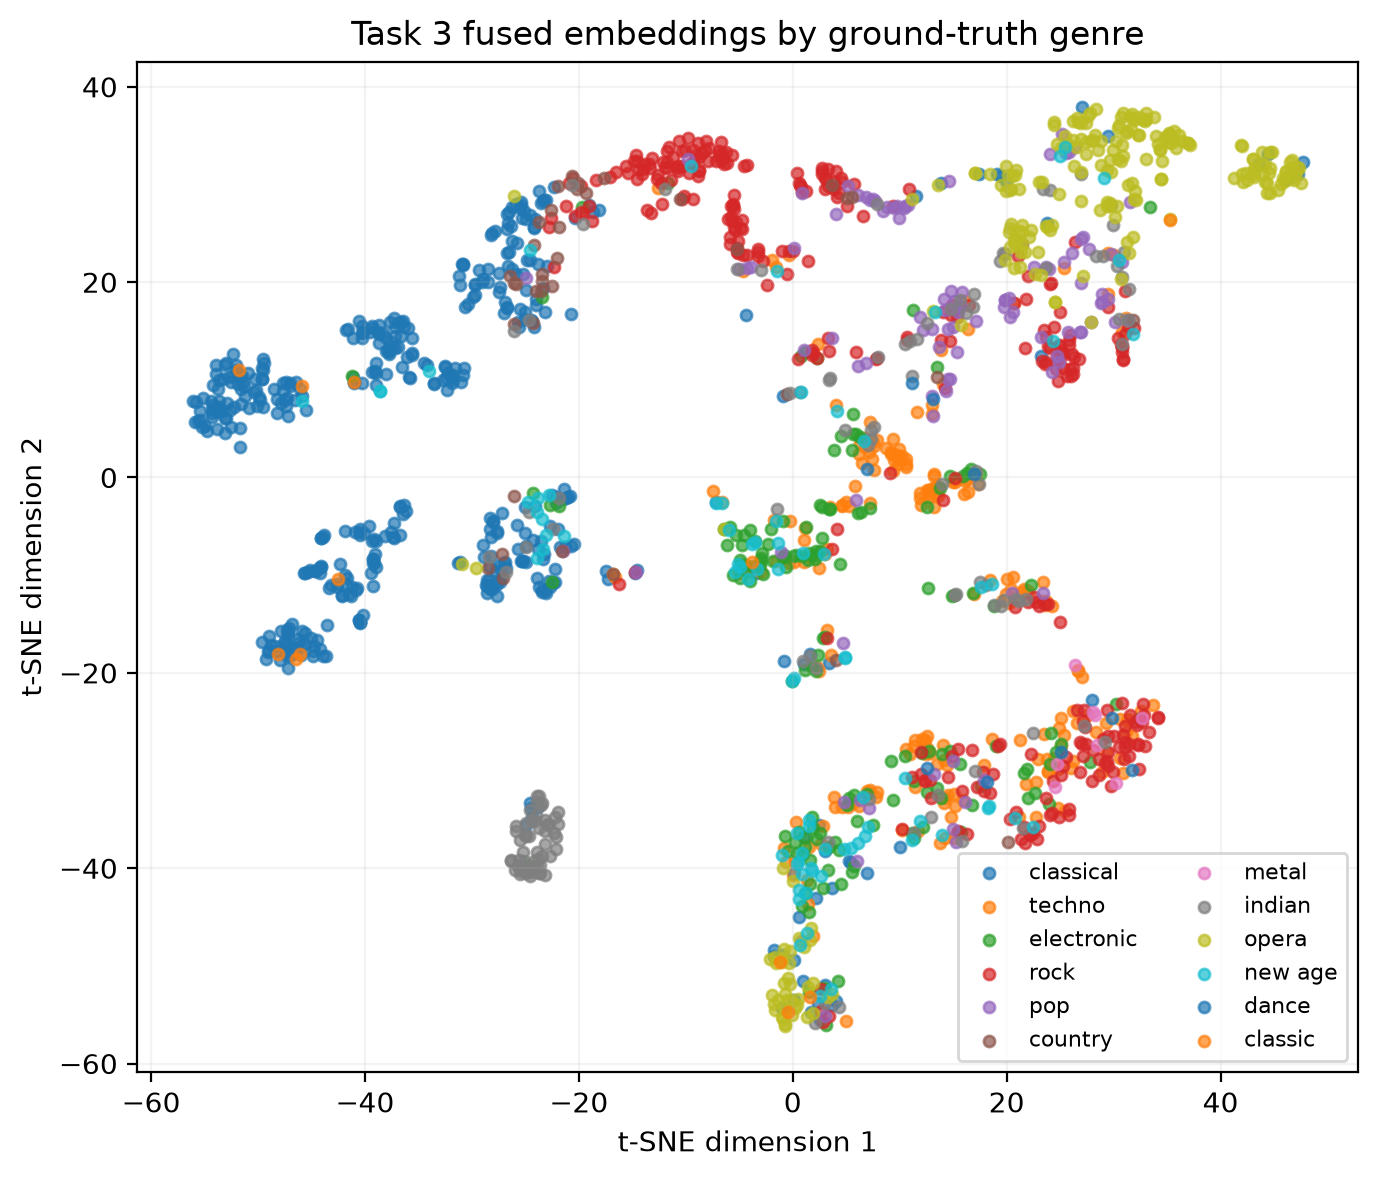
\includegraphics[width=\linewidth]{task3_tsne_genre.png}\\[2pt]
    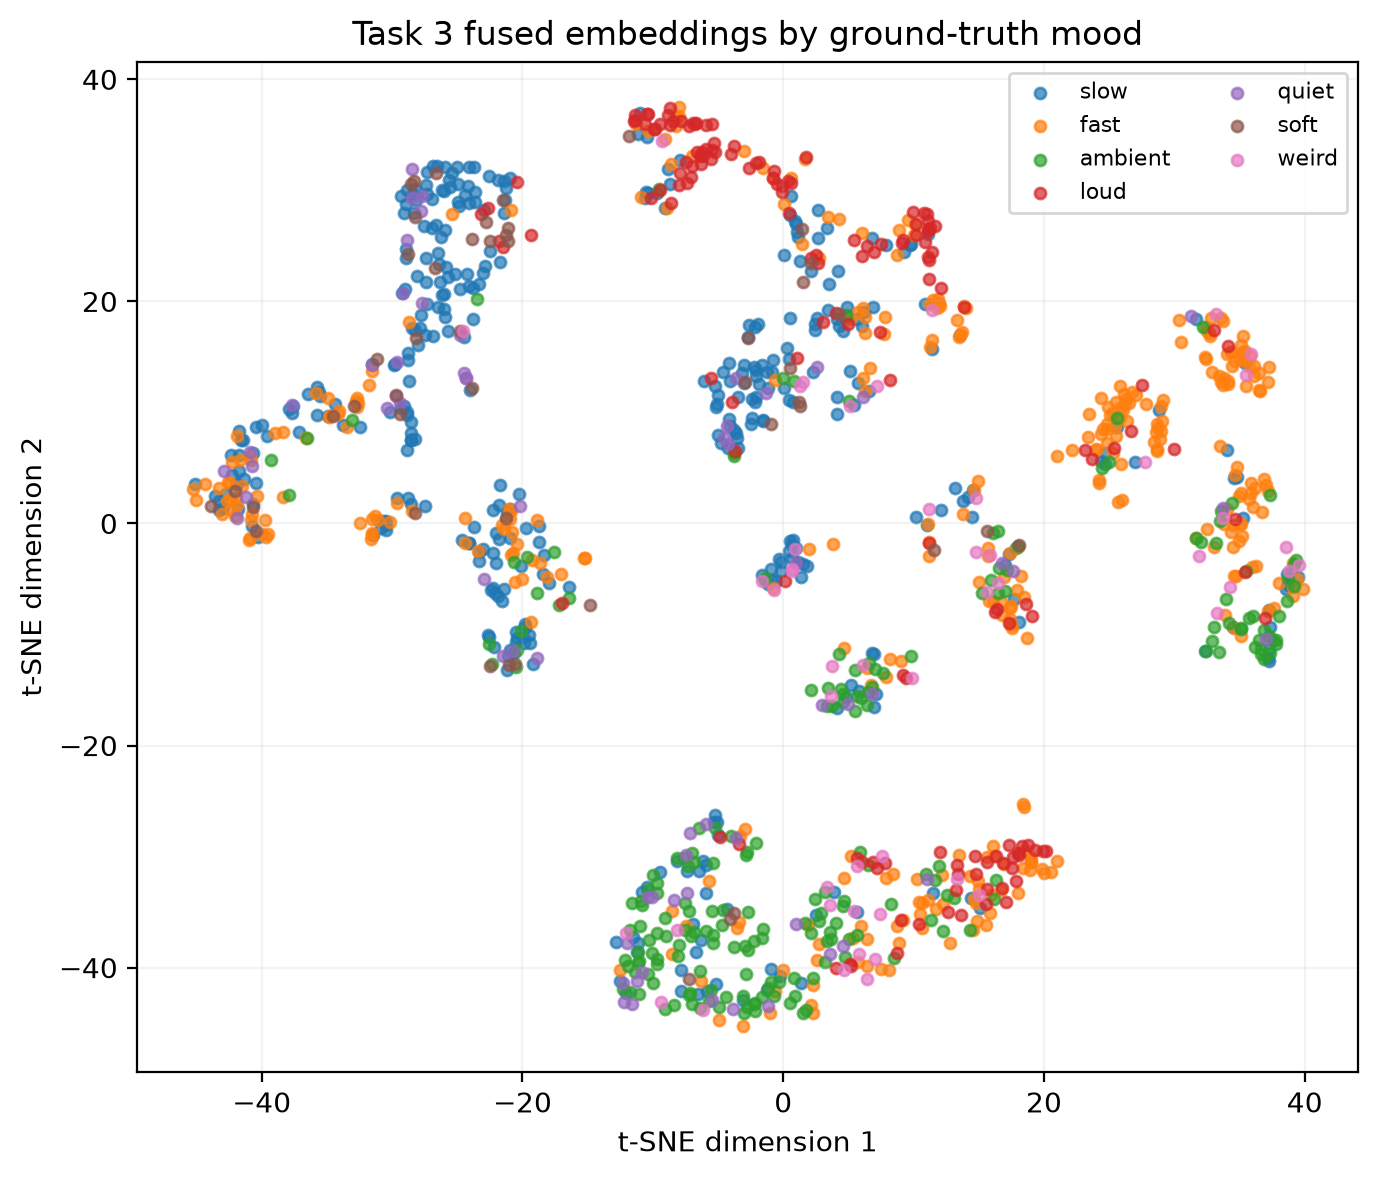
\includegraphics[width=\linewidth]{task3_tsne_mood.png}
  \end{minipage}
  \caption{Task 3 diagnostics: held-out per-tag scores (left) and ground-truth-labelled
  genre/mood t-SNE views (right).}
\end{figure*}}{}
\FloatBarrier

\subsection{Task 4}
\IfFileExists{../plots/task4_learning_curve.png}{
\begin{figure}[t]
  \centering
  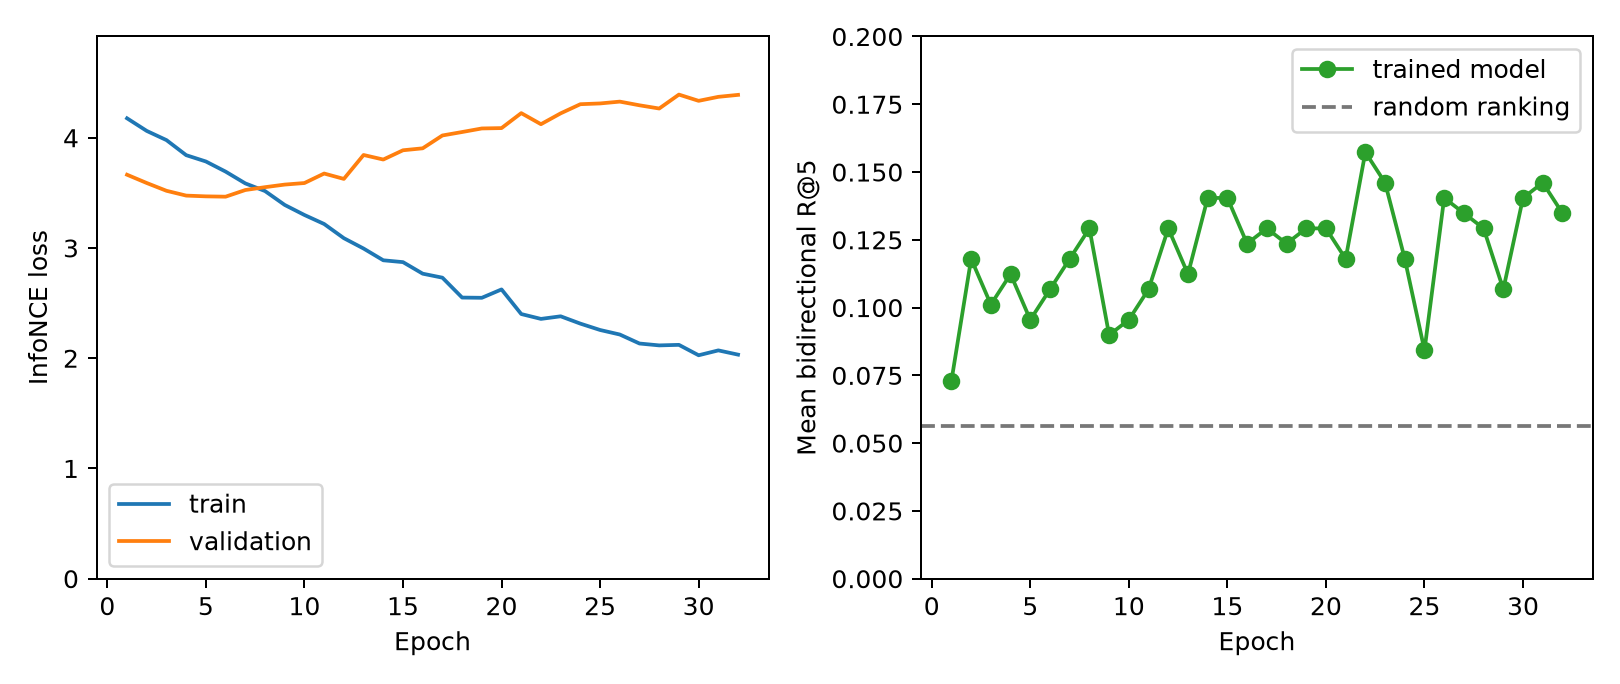
\includegraphics[width=\columnwidth]{task4_learning_curve.png}\\[-2pt]
  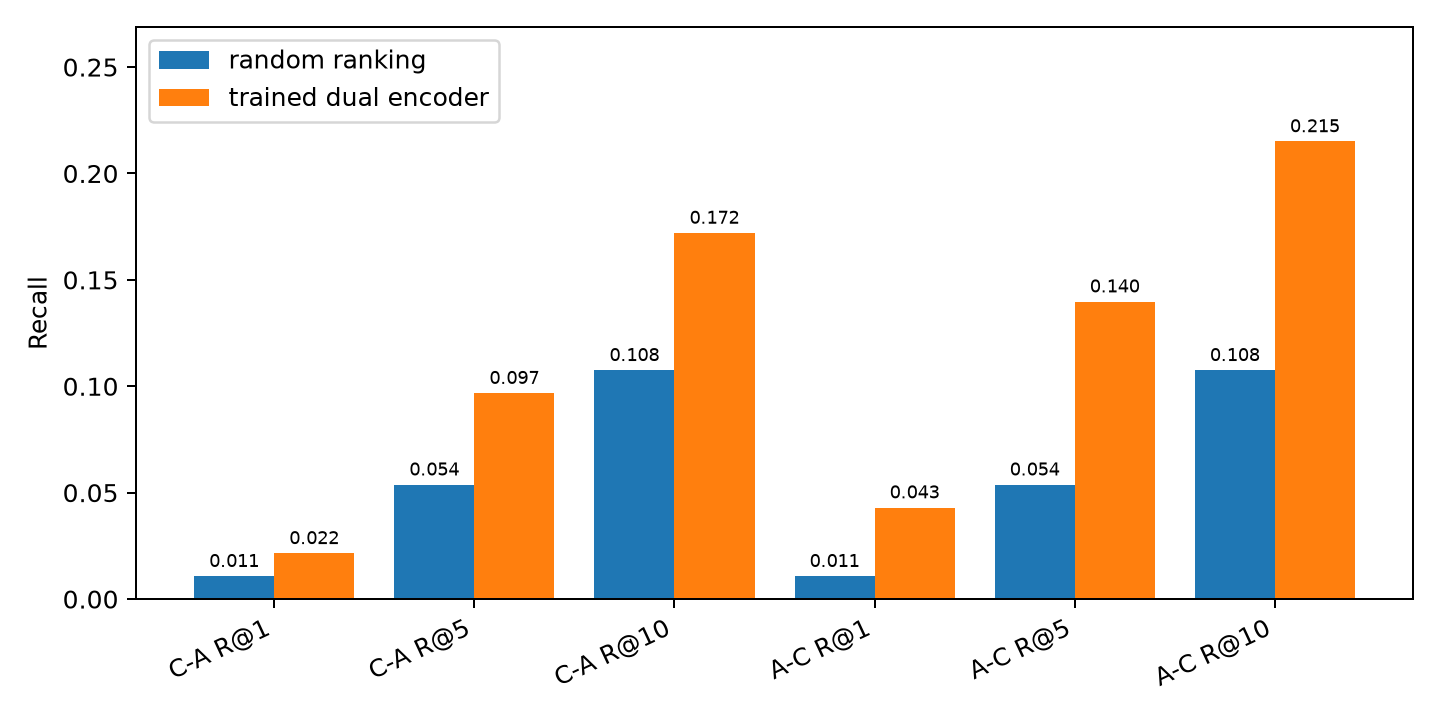
\includegraphics[width=\columnwidth]{task4_retrieval_recall.png}
  \caption{Task 4 optimization (top) and held-out bidirectional retrieval compared with random
  ranking (bottom).}
\end{figure}}{}

The selected contrastive checkpoint is from epoch \TaskFourBestEpoch{}. Caption-to-audio
Recall@1/5/10 is \TaskFourCtoAOne{}/\TaskFourCtoAFive{}/\TaskFourCtoATen{}, and
audio-to-caption Recall@1/5/10 is
\TaskFourAtoCOne{}/\TaskFourAtoCFive{}/\TaskFourAtoCTen{}. Random-ranking Recall@5 for this
test size is \TaskFourRandomFive{}. The learning plot separates loss from retrieval recall and
starts both vertical axes at zero, so changes remain readable without a misleading dual axis.


\section{Qualitative Analysis}
Three supplementary cases use real held-out MusicCaps intervals and their expert captions. The
MTAT-trained cross-attention checkpoint is applied without additional MusicCaps tuning. Each panel
shows the temporal segment path, any similarity edges passing the fixed threshold, and the caption
tokens receiving the most mean cross-attention. These visualizations are a qualitative transfer check,
not a MusicCaps performance estimate or a causal explanation.

Task 4 additionally saves ten held-out captions with their top three retrieved audio clips.
These examples preserve the clip IDs, source intervals, similarity scores, and whether the paired
clip was retrieved. For the requested zero-shot comparison, caption and 19 tag-prompt embeddings
are matched without Task 4 tag supervision. Its Macro-F1 is \TaskFourZeroShotMacro{}, compared
with \TaskFourTaskThreeMacro{} when the supervised Task 3 cross-attention classifier is transferred
directly to the same MusicCaps examples. Both are transfer checks because the available
MusicCaps aspects are only an imperfect match to the MTAT target vocabulary.

\IfFileExists{../plots/task3_musiccaps_case_studies.png}{
\begin{figure*}[t]
  \centering
  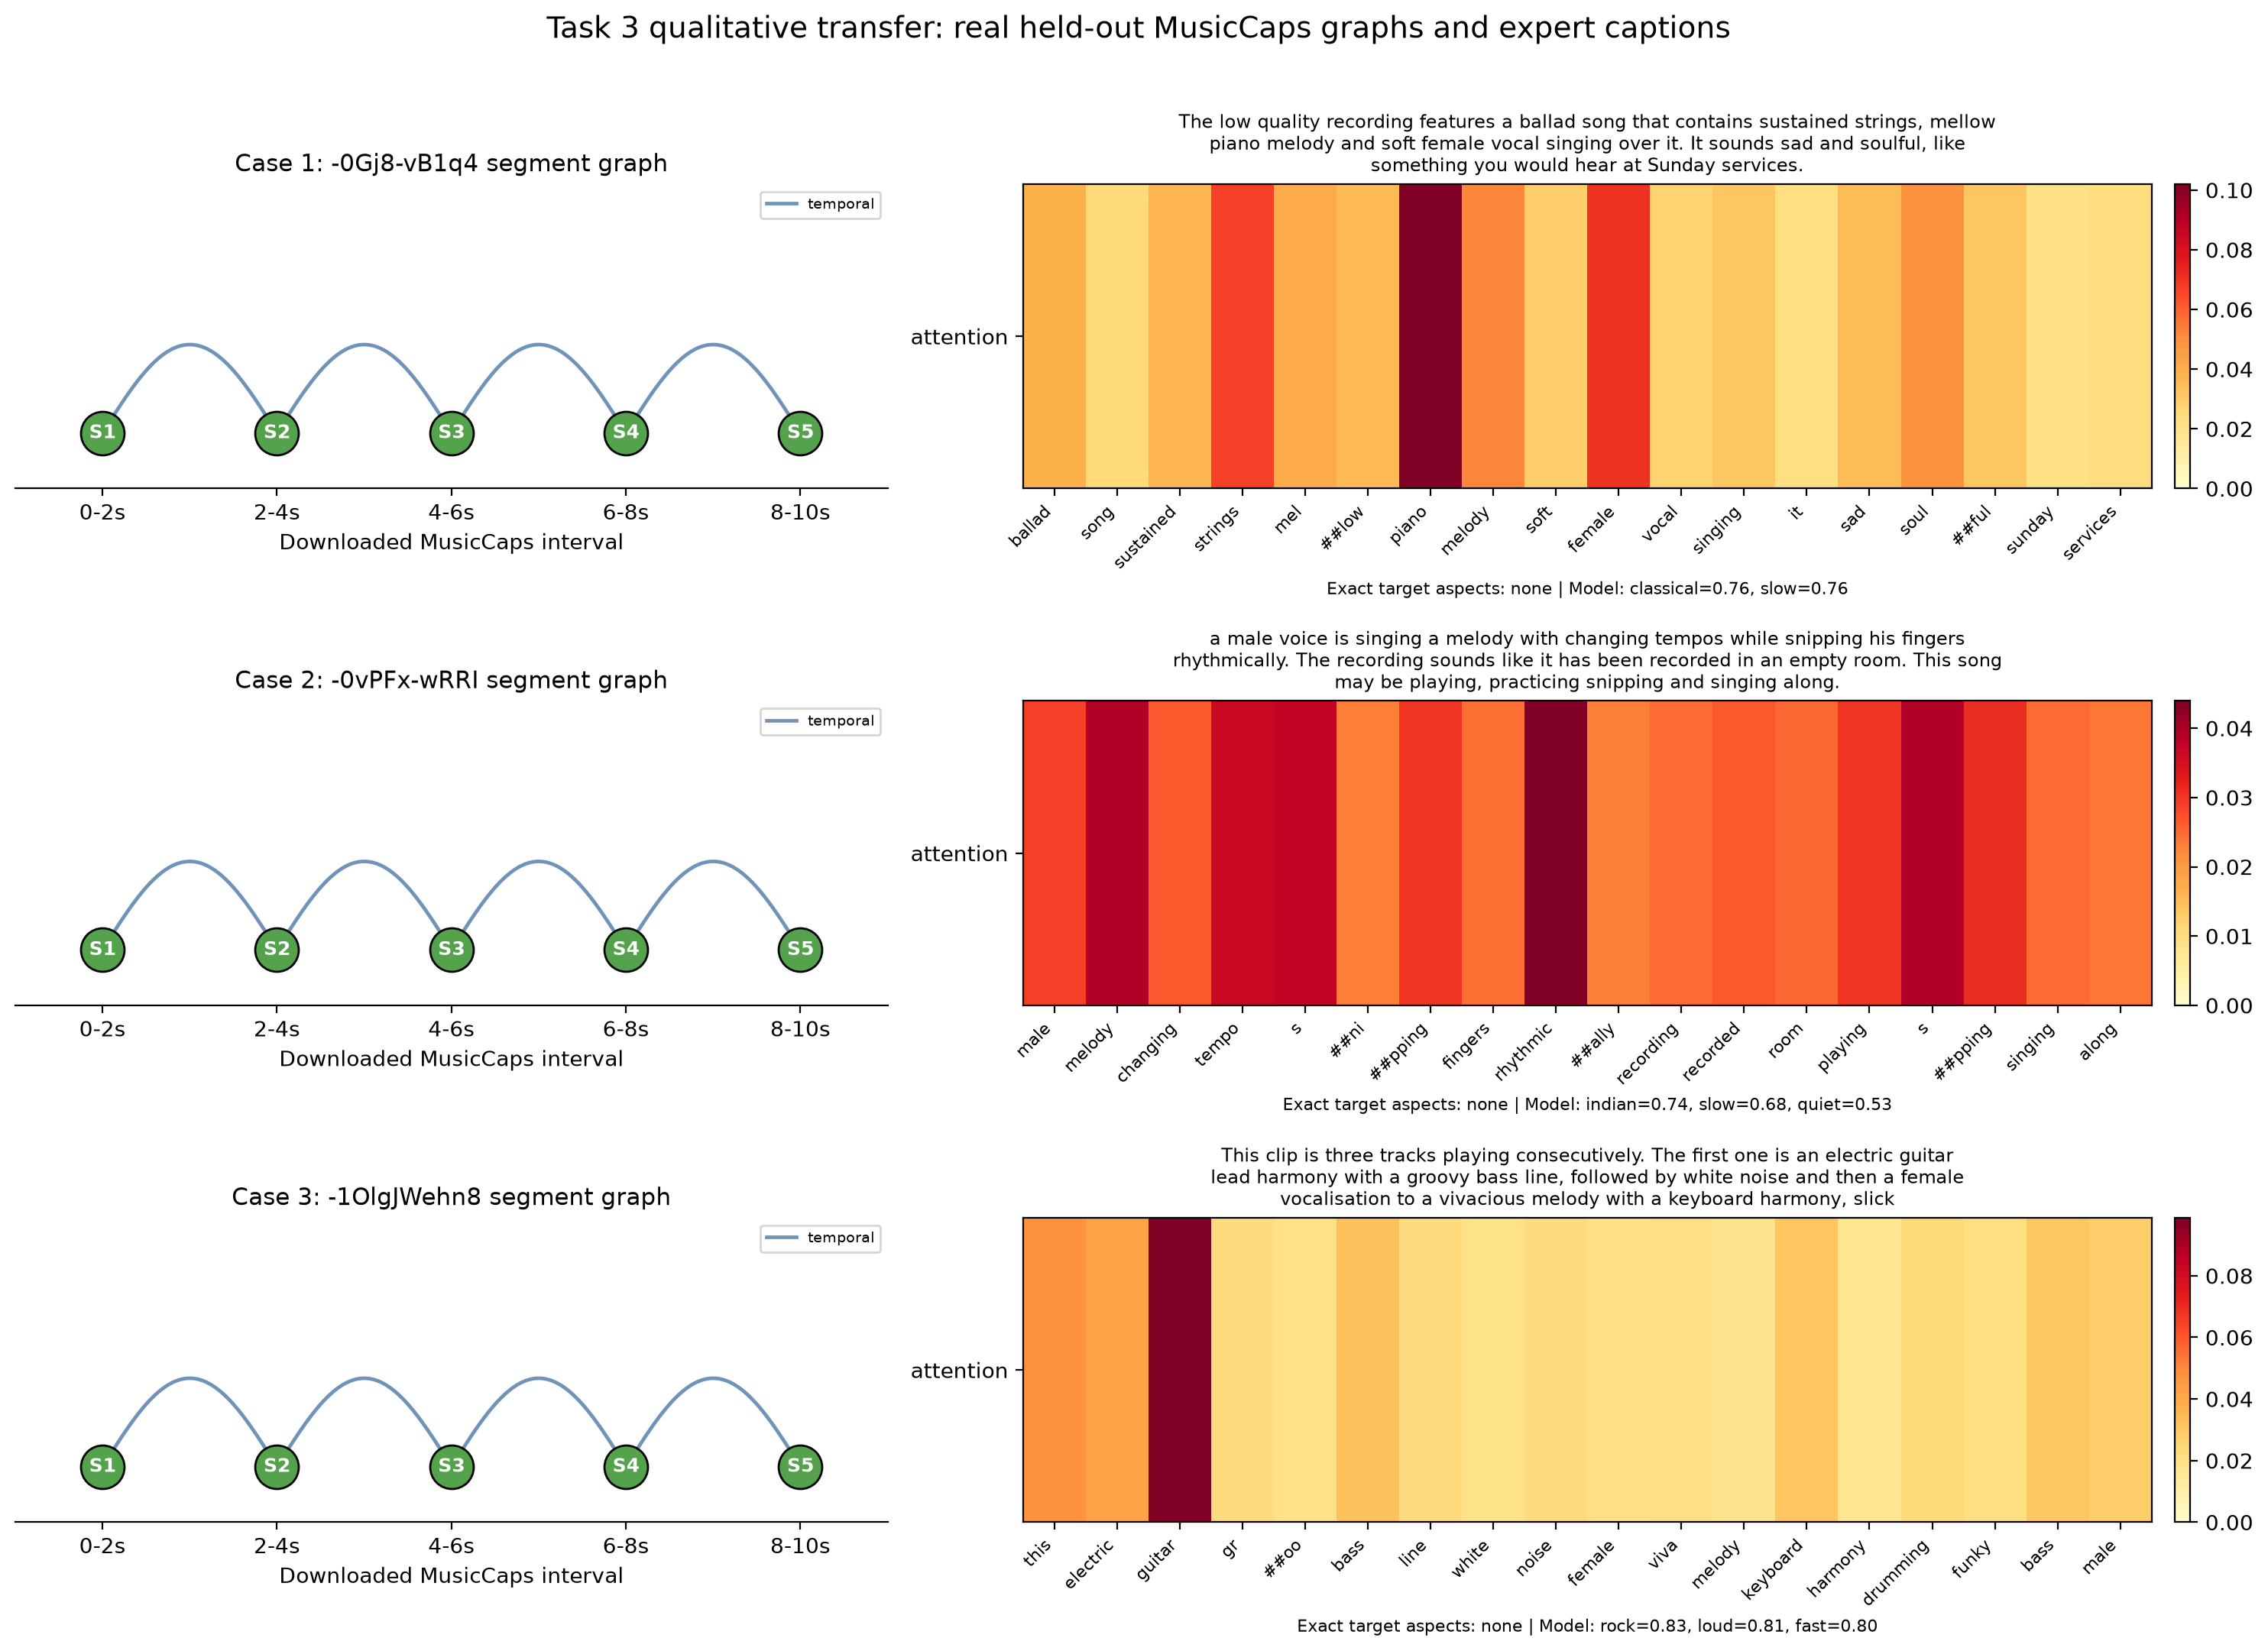
\includegraphics[width=.90\textwidth]{task3_musiccaps_case_studies.png}
  \caption{Three deterministic held-out MusicCaps graph/caption alignment cases. Only the 18
  highest-attention content tokens are displayed, in their original sequence order.}
\end{figure*}}{}
\FloatBarrier


\section{Limitations and Responsible Use}
MagnaTagATune tags are noisy and were collected through a game. Context and target tags are
disjoint in wording but are not independent. Artist overlap also remains in the official shard
split. MusicCaps captions contain subjective descriptions, and YouTube availability can change
the usable Task 4 sample. The contrastive experiment therefore represents a fixed recovered
subset, not the complete MusicCaps benchmark. GTZAN is small and contains known data-quality
concerns. For these
reasons, the models should be treated as course experiments rather than general-purpose music
understanding systems.

The project processes only public research datasets. Audio is not redistributed in the source
repository. Generated predictions may reflect dataset biases and should not be used to make
decisions about artists or listeners.

\section{Conclusion}
This project implements text-only, graph-only, and multimodal music-context models in a common
PyTorch pipeline. On GTZAN, the CNN clearly outperforms GraphSAGE, showing that the 77-D segment
summaries discard information retained by the full mel spectrogram. On MTAT, both multimodal
models outperform their single-modality ablations, and early concatenation gives the strongest
overall result. Cross-attention remains competitive but does not beat the simpler fusion method.
The real-audio contrastive extension also supplies bidirectional retrieval, ten top-three
examples, and a zero-shot tag-transfer check; its scores are interpreted against random ranking
rather than presented as benchmark performance.
Frozen splits, validation-only selection, duplicate audits, saved checkpoints, and generated
tables make these findings reproducible without overstating them.

\begin{thebibliography}{9}
\bibitem{bert} J. Devlin, M.-W. Chang, K. Lee, and K. Toutanova, ``BERT: Pre-training of deep
bidirectional transformers for language understanding,'' in \emph{NAACL-HLT}, 2019.
\bibitem{distilbert} V. Sanh, L. Debut, J. Chaumond, and T. Wolf, ``DistilBERT, a distilled
version of BERT: smaller, faster, cheaper and lighter,'' 2019.
\bibitem{graphsage} W. Hamilton, Z. Ying, and J. Leskovec, ``Inductive representation learning
on large graphs,'' in \emph{NeurIPS}, 2017.
\bibitem{gtzan} G. Tzanetakis and P. Cook, ``Musical genre classification of audio signals,''
\emph{IEEE Transactions on Speech and Audio Processing}, 2002.
\bibitem{mtat} E. Law, K. West, M. Mandel, M. Bay, and J. Downie, ``Evaluation of algorithms
using games: The case of music tagging,'' in \emph{ISMIR}, 2009.
\bibitem{pyg} M. Fey and J. E. Lenssen, ``Fast graph representation learning with PyTorch
Geometric,'' in \emph{ICLR Workshop}, 2019.
\end{thebibliography}

\end{document}
